\documentclass[a4paper,12pt]{article}

\usepackage[utf8]{inputenc}
\usepackage[left=0.5in,right=0.5in,top=1in,bottom=1in]{geometry}
\usepackage{amsmath,amssymb,amsfonts,mathtools}
\usepackage{pgfplots,graphicx,calc,changepage}
\pgfplotsset{compat=newest}
\usepackage{enumitem}
\usepackage{fancyhdr}
\usepackage[colorlinks = true, linkcolor = blue]{hyperref}

% Syntax highlighting
\usepackage{listings}
\usepackage{xcolor}

\definecolor{codegreen}{rgb}{0.40,0.62,0.07}
\definecolor{codegray}{rgb}{0.5,0.5,0.5}
\definecolor{codeblue}{rgb}{0.09,0.57,0.73}
\definecolor{backcolour}{rgb}{1,1,1}

\lstdefinestyle{mystyle}{
    backgroundcolor=\color{backcolour},   
    commentstyle=\color{codegreen},
    keywordstyle=\color{magenta},
    numberstyle=\tiny\color{codegray},
    stringstyle=\color{codeblue},
    basicstyle=\ttfamily\small,
    breaklines=true,                     
    keepspaces=true,                 
    numbers=left,                    
    numbersep=5pt,                  
    showspaces=false,
    showstringspaces=false,
    showtabs=false,                  
    tabsize=4
}

\lstset{style=mystyle}

\newcommand{\nats}{\mathbb{N}}
\newcommand{\reals}{\mathbb{R}}
\newcommand{\rats}{\mathbb{Q}}
\newcommand{\ints}{\mathbb{Z}}
\newcommand{\comps}{\mathbb{C}}
\newcommand{\pols}{\mathcal{P}}
\newcommand{\cants}{\Delta\!\!\!\!\Delta}
\newcommand{\eps}{\varepsilon}
\newcommand{\st}{\backepsilon}
\newcommand{\abs}[1]{\left| #1 \right|}
\newcommand{\dom}[1]{\mathrm{dom}\left(#1\right)}
\newcommand{\for}{\text{ for }}
\newcommand{\dd}[1]{\mathrm{d}#1}
\newcommand{\spn}{\mathrm{sp}}
\newcommand{\nul}{\mathcal{N}}
\newcommand{\col}{\mathrm{col}}
\newcommand{\rank}{\mathrm{rank}}
\newcommand{\norm}[1]{\lVert #1 \rVert}
\newcommand{\inner}[1]{\left\langle #1 \right\rangle}
\newcommand{\pmat}[1]{\begin{pmatrix} #1 \end{pmatrix}}
\renewcommand{\and}{\text{ and }}

\newsavebox{\qed}
\newenvironment{proof}[2][$\square$]
    {\setlength{\parskip}{0pt}\par\textit{Proof:} #2\setlength{\parskip}{0.25cm}
        \savebox{\qed}{#1}
        \begin{adjustwidth}{\widthof{Proof:}}{}
    }
    {
        \hfill\usebox{\qed}\end{adjustwidth}
    }

\pagestyle{fancy}
\fancyhead{}
\lhead{Caleb Jacobs}
\chead{APPM 5600: Numerical Analysis I}
\rhead{Homework \#8}
\cfoot{}
\setlength{\headheight}{35pt}
\setlength{\parskip}{0.25cm}
\setlength{\parindent}{0pt}

\begin{document}
\section*{Problems}
\begin{enumerate}[label = \arabic*.]
	\item \
		\begin{enumerate}[label = (\roman*)]
			\item Given $ x_0 = -0.2, x_1 = 0, $ and $ x_2 = 0.2 $ construct a second degree polynomial to approximate $ f(x) = e^x $ via Newton's divided differences.
			
			We want to derive a polynomial of the form
			\[
				p(x) = a_0 + a_1 (x - x_0) + a_2 (x - x_0)(x - x_1)
			\]
			where $ a_i = [x_0, \ldots, x_{i-1}] $ are the Newton Divided differences. For this problem, we have
			\begin{align*}
				a_0 &= f[x_0] = e^{x_0} = e^{-0.2}, \\
				a_1 &= f[x_0, x_1] = \frac{e^{x_1} - e^{x_0}}{x_1 - x_0} = \frac{1 - e^{-0.2}}{0.2},\\
				\shortintertext{and} \\
				a_2 &= f[x_0, x_1, x_2] = \frac{f[x_1, x_2] - f[x_0, x_1]}{x_2 - x_0} = \frac{\frac{e^{0.2} - 1}{0.2} - \frac{1 - e^{-0.2}}{0.2}}{0.4}
			\end{align*}
			which makes our polynomial
			\begin{align*}
				p(x) &= e^{-0.2} + \frac{1 - e^{-0.2}}{0.2}(x + 0.2) + \frac{\frac{e^{0.2} - 1}{0.2} - \frac{1 - e^{-0.2}}{0.2}}{0.4} (x + 0.2)(x) \\
				&= 1 + 1.00668 x + 0.501669 x^2.
			\end{align*}
			
			\item Derive an error bound for $ p_2(x) $ when $ x \in [-0.2, 0.2] $.
			
			First, note that the third derivative of $ f $ is maximized over $ [-0.2,0.2] $ when $ x = 0.2 $. Then, we can obtain a bound on our error as
			
			\begin{align*}
				E(t) &\leq \max_{t \in [-0.2, 0.2]} E(t) \\
				&= \max_{t \in [-0.2, 0.2]} \frac{(t + 0.2)(t)(t - 0.2)}{6} e^{0.2} \\
				&= \frac{(-\frac{\sqrt{3}}{15} + 0.2)(-\frac{\sqrt{3}}{15})(-\frac{\sqrt{3}}{15} - 0.2)}{6} e^{0.2} \\
				&= 6.26824 \cdot 10^{-4}.
			\end{align*}
			
			\item Compute the error $ E(0.1) = f(0.1) - p_2(0.1) $. How does this compare with the error bound?
			
			Our error is
			\[
				E(0.1) = \abs{1.10517 - 1.10568} = 5.136621 \cdot 10^{-4}
			\]
			which is within our error bound! So our error bound holds $ x = 0.1 $.
		\end{enumerate}
	
	\newpage
	\item \
		\begin{enumerate}[label = (\roman*)]
			\item Show there is a unique cubic polynomial $ p(x) $ for which 
			\begin{align*}
				p(x_0)  &= f(x_0) & p(x_2)   &= f(x_2) \\
				p'(x_1) &= f'(x_1) & p''(x_1) &= f''(x_1)
			\end{align*}
			where $ f(x) $ is a given function and $ x_0 \neq x_2 $.
			
			Suppose $ p(x) $ and $ q(x) $ are two cubic polynomials satisfying
			\begin{align*}
				p(x_0) = q(x_0)  &= f(x_0) & p(x_2) = q(x_2)    &= f(x_2) \\
				p'(x_1) = q(x_1) &= f'(x_1) & p''(x_1) = q''(x_1) &= f''(x_1).
			\end{align*}
			Now let $ v(x) + p(x) - q(x) $. Then, by linearity, $ v(x) $ is a cubic polynomial that satisfies
			\begin{align*}
				v(x_0)  &= 0 & v(x_2)  &= 0 \\
				v'(x_1) &= 0 & v''(x_1) &= 0.
			\end{align*}
			Furthermore, because $ v(x) $ is a cubic polynomial, there exists constants $ a_0, a_1, a_2, $ and $ a_3 $ such that
			\begin{align*}
				v(x)   &= a_0 + a_1 x + a_2 x^2 + a_3 x^3 \\
				v'(x)  &= a_1 + 2 a_2 x + 3 a_3 x^2 \\
				v''(x) &= 2 a_2 + 6 a_3 x.
			\end{align*}
			Then,
			\[
				v''(x_1) = 2 a_2 + 6 a_3 x_1 = 0
			\]
			which implies
			\[
				a_2 = -3a_3.
			\]
			Using this expression in our first derivative yields
			\[
				v'(x_1) = a_1 - 6 a_3 x_1^2 + 3 a_3 x_1^2 = 0
			\]
			which implies
			\[
				a_1 = 3 a_3 x_1^2.
			\]
			Finally, 
			\begin{align*}
				v(x) &= a_0 + 3a_3 x_1^2 x - 3 a_3 x_1 x^2 + a_3 x^3 \\
				&= a_0 + 3a_3 x_1^2 x - 3 a_3 x_1 x^2 + a_3 x^3 - a_3 x_1^3 + a_3 x_1^3 \\
				&= (a_0 + a_3 x_1^3) - a_3 (x - x_1)^3.
			\end{align*}
			Then, using our last constraints, we have the system
			\begin{align*}
				v(x_0) &= (a_0 + a_3 x_1^3) - a_3 (x_0 - x_1)^3 = 0 \\
				v(x_2) &= (a_0 + a_3 x_1^3) - a_3 (x_2 - x_1)^3 = 0
			\end{align*}
			which yields
			\[
				a_3 (x_0 - x_1)^3 = a_3(x_2 - x_1)^3.
			\]	
			Then, because $ x_0 \neq x_2 $, we must have $ a_3 = 3 $ which implies $ a_0 = 0 $. Therefore,
			\[
				v(x) = 0
 			\]
 			and so we must have
 			\[
 				p(x) = q(x)
 			\]
 			showing the uniqueness of our polynomial.
								
			\item Derive a formula for $ p(x) $.
			
			We know $ p(x) $ has the form
			\[
				p(x) = a_0 + a_1 x + a_2 x^2 + a_3 x^3
			\]
			for some constants $ a_0, a_1, a_2, $ and $ a_3 $. Then, using our second derivative information, we have
			\[
				p''(x_1) = 2 a_2 + 6a_3 x_1 = f''(x_1)
			\]
			which implies 
			\[
				a_2 = \frac{1}{2} f''(x_1) - 3 a_3 x_1.
			\]
			Then, using our first derivative information, we have
			\[
				p'(x_1) = a_1 + 2\left(\frac{1}{2} f''(x_1) - 3a_3 x_1\right) x_1 + 3a_3 x_1^2 = f'(x_1)
			\]
			which implies 
			\[
				a_1 = f'(x_1) - f''(x_1)x_1 + 3 a_3 x_1^2.
			\]
			Next, we can use our function information to get the system
			\begin{align*}
				p(x_0) &= a_0 + f'(x_1)x_0 - f''(x_1) x_0 x_1 + 3a_3 x_0 x_1^2 + \frac{1}{2} f''(x_1)x_0^2 - 3a_3 x_0^2 x_1 + a_3 x_0^3 = f(x_0) \\
				p(x_2) &= a_0 + f'(x_1)x_2 - f''(x_1) x_1 x_2 + 3a_3 x_1^2 x_2 + \frac{1}{2} f''(x_1)x_2^2 - 3a_3 x_1 x_2^2 + a_3 x_2^3 = f(x_2)
				\shortintertext{which implies}
				a_3 &= \frac{f(x_2) - f(x_0) + f'(x_1)(x_0 - x_2) - f''(x_1) x_1(x_0 - x_2) + \frac{1}{2} f''(x_1) (x_0^2 - x_2^2)}{3 x_1^2 (x_2 - x_0) + 3x_1 (x_0^2 - x_2^2) + x_2^3 - x_0^3} \\
				a_0 &= f(x_0) - f'(x_1)x_0 + f''(x_1) x_0 x_1 + 3a_3 x_0 x_1^2 - \frac{1}{2} f''(x_1)x_0^2 + 3a_3 x_0^2 x_1 - a_3 x_0^3.
			\end{align*}
			Now, we construct our polynomial by first computing $ a_3, a_0, a_1, $ and $ a_2 $ in that order and then plugging them into our polynomial
			\[
				p(x) = a_0 + a_1 x + a_2 x^2 + a_3 x^3.
			\]
			
			
			\item Let $ x_0 = -1, x_1 = 0, $ and $ x_2 = 1 $. Assuming $ f(x) \in C^4[-1,1] $, show that for $ x \in [-1,1] $,
			\[
				f(x) - p(x) = \frac{x^4 - 1}{4!}f^4(\eta_x)
			\]
			for some $ \eta_x \in [-1,1] $.
			
			Suppose we have a fixed $ t \in [-1,1] $ such that $ t \neq x_0 $ and $ t \neq x_2 $. Next, define
			\[
				G(x) = E(x) - \frac{x^4 - 1}{t^4 - 1} E(t)
			\]
			where $ E(x) = f(x) - p(x) $. Then, by construction, we have $ G(x_0) = G(x_2) = G(t) = 0 $. Next, using Rolle's theorem, we have must have at least two roots to $ G'(x) $. But, $ G'(x_1) = 0 $ by construction and so as long as the two roots from Rolle's theorem do not coincide with $ x_1 $, $ G'(x) $ has three roots (Note it is highly unlikely that $ x_1 $ will be the point given from Rolle's theorem). Then, using Rolle's theorem again implies that $ G''(x) $ also has two roots that are not equal to $ x_1 $. So, because $ G''(x_1) = 0 $, we know $ G''(x) $ also has at least three roots. Using Rolle's theorem twice more tells us that $ G^{(3)}(x) $ has two roots which implies $ G^{(4)}(x) $ has one root; call this root $ \eta_x \in [-1,1] $. Then, we have
			\begin{align*}
				G^{(4)} &= E^{(4)}(\eta_4) - \frac{4!}{t^4 - 1} E(t) \\
				&= f^{(4)}(\eta_x) - \frac{4!}{t^4 - 1} E(t) = 0
			\end{align*}
			which implies
			\[
				E(t) = \frac{t^4 - 1}{4!} f^{(4)}(\eta_x).
			\]
			Then, if we rename $ t $ to $ x $, we have
			\[
				E(x) = f(x) - p(x) = \frac{x^4 - 1}{4!} f^{(4)}(\eta_x).
			\]
			
		\end{enumerate}
	 \newpage
	\item Suppose we have $ m $ data points $ \{(t_i, y_i)\}_{i = 1}^m $, where the $ t $-values all occur in some interval $ [x_0, x_n] $. We subdivide the interval $ [x_0, x_n] $ into $ n $ subintervals $ \{[x_k, x_{k + 1}]_{k = 0}^{n - 1}\} $ of equal length $ h $ and attempt to choose a spline function $ s(x) $ with nodes at $ \{x_k\}_{k = 0}^n $ in such a way so that
	\[
		\sum_{i = 1}^{m} \abs{y_i - s(t_i)}^2
	\]
	is \emph{minimized}.
		\begin{enumerate}[label = (\roman*)]
			\item My B-Spline code is given at the end of the document
			
			\item Using my code, I was able to produce the following noisy plots:
			\begin{figure}[h!]
				\centering
				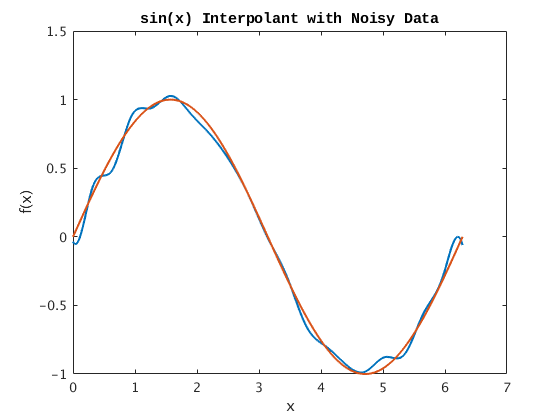
\includegraphics[width = 0.45\textwidth]{images/sin.png}
				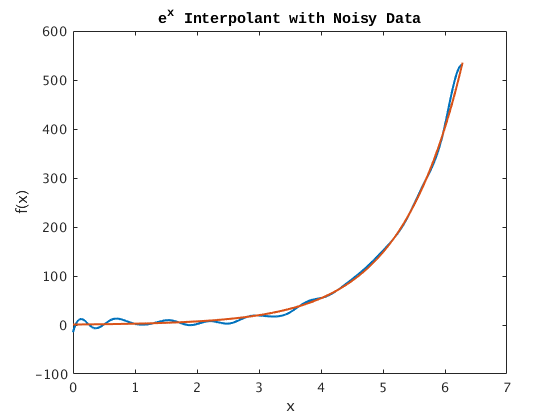
\includegraphics[width = 0.45\textwidth]{images/exp.png}
				
				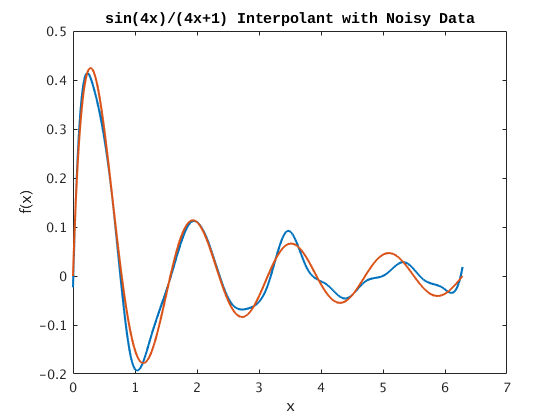
\includegraphics[width = 0.45\textwidth]{images/sinc.png}
			\end{figure}
			
			\newpage
			\item My spy plot is given below. We can see that we have nice and relatively uniform sparse structure throughout the matrix. Each row has at most 4 nonzero entries that are all consecutive. Furthermore, each new row either shifts the 4 consecutive non entries to the right by 1 or not at all. 
			\begin{figure}[h!]
				\centering
				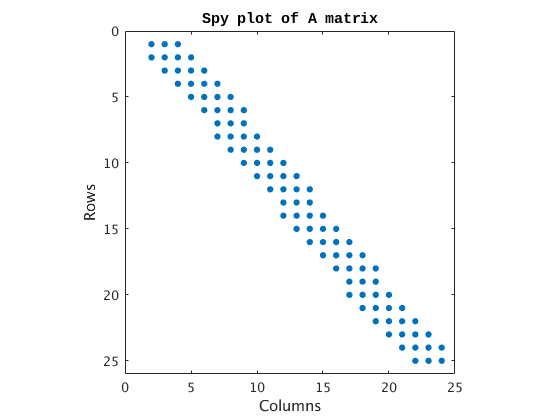
\includegraphics[width = 0.6\textwidth]{images/spy.png}
			\end{figure}
		\end{enumerate}
\end{enumerate}

\newpage
\section*{Code Used}
\rule{\textwidth}{0.4pt}
	\lstinputlisting[language = matlab]{code/B_Splines.m}
\rule{\textwidth}{0.4pt}
\end{document}